\documentclass[border=5mm]{standalone}
\usepackage{tikz}
\usepackage{amsmath, amssymb}\usetikzlibrary{positioning}
\usepackage{graphicx}


\begin{document}

% Coordinate map: hidden states run left to right at y=1, with their inputs
% directly below at y=-0.8 and their outputs directly above at y=2.9.
% Ellipses on either side indicate time steps omitted from this excerpt.
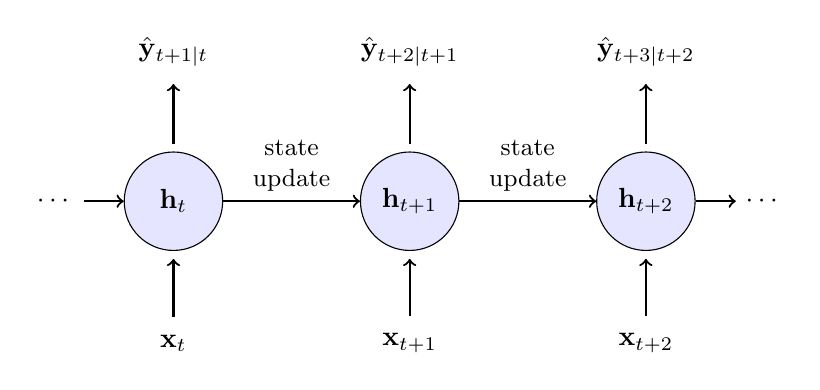
\begin{tikzpicture}[
          neuron/.style={circle, draw, minimum size=1.25cm, inner sep=0pt, fill=blue!10},
          arrow/.style={->, thick},
          node distance=0.5cm
        ]
          % RNN cells
          \node[neuron] (h1) at (0,1) {$\mathbf{h}_t$};
          \node[neuron] (h2) at (3,1) {$\mathbf{h}_{t+1}$};
          \node[neuron] (h3) at (6,1) {$\mathbf{h}_{t+2}$};
          \node (past) at (-1.5,1) {$\cdots$};
          \node (future) at (7.5,1) {$\cdots$};

          % Inputs
          \node (x1) at (0,-0.8) {$\mathbf{x}_t$};
          \node (x2) at (3,-0.8) {$\mathbf{x}_{t+1}$};
          \node (x3) at (6,-0.8) {$\mathbf{x}_{t+2}$};

          % Outputs
          \node (y1) at (0,2.9) {$\hat{\mathbf{y}}_{t+1\mid t}$};
          \node (y2) at (3,2.9) {$\hat{\mathbf{y}}_{t+2\mid t+1}$};
          \node (y3) at (6,2.9) {$\hat{\mathbf{y}}_{t+3\mid t+2}$};

          % Arrows
          \draw[arrow, shorten >=1mm, shorten <=1mm] (x1.north) -- (h1.south);
          \draw[arrow, shorten >=1mm, shorten <=1mm] (x2.north) -- (h2.south);
          \draw[arrow, shorten >=1mm, shorten <=1mm] (x3.north) -- (h3.south);

          \draw[arrow, shorten >=1mm, shorten <=1mm] (h1.north) -- (y1.south);
          \draw[arrow, shorten >=1mm, shorten <=1mm] (h2.north) -- (y2.south);
          \draw[arrow, shorten >=1mm, shorten <=1mm] (h3.north) -- (y3.south);

          \draw[arrow] (past.east) -- (h1.west);
          \draw[arrow] (h1) -- node[above, align=center, font=\small] {state\\update} (h2);
          \draw[arrow] (h2) -- node[above, align=center, font=\small] {state\\update} (h3);
          \draw[arrow] (h3.east) -- (future.west);
        \end{tikzpicture}

    \end{document}
